\chapter{Teknik Laboratorium I: Keselamatan, Pengukuran, dan Pemisahan}\label{ch:b1:lab-techniques-1}

Dua mahasiswa merekristalisasi aspirin dari bets yang sama dan mengukur
titik lelehnya pada bangku pemanas yang sama. Yang satu membaca
\qty{134}{\celsius}, yang lain \qty{136}{\celsius}. Apakah keduanya
berselisih? Apakah produknya murni? Tidak satu pun dari kedua pertanyaan
itu dapat dijawab hanya dari dua angka itu: sebuah pengukuran baru
bernilai jika disertai ketidakpastiannya, dan sebuah perbandingan baru
bernilai jika disertai sebuah aturan. Bab terakhir ini menghimpun sisi
praktis tahun ini: cara membaca \omterm{def:b1:lab-techniques-1:hazard}{bahaya} dari apa yang ada di atas meja
kerja, cara menyatakan nilai terukur beserta ketidakpastiannya dan
membandingkannya dengan nilai lain, dan cara operasi-operasi klasik
laboratorium organik --- ekstraksi, penyaringan, \omterm{def:b1:lab-techniques-1:recrystallisation}{rekristalisasi},
distilasi --- memisahkan sebuah produk dari zat-zat di sekitarnya, lalu
memeriksa kemurniannya.

\begin{recall}
\omterm{def:b1:precipitation:solubility}{Kelarutan} dan ketercampuran berdasarkan gaya antarmolekul, \omterm{def:b1:intermolecular-forces-solvents:solvent-classes}{pelarut polar}
dan apolar (\cref{ch:b1:intermolecular-forces-solvents}); buret, pipet,
dan \omterm{def:b1:titration-methods:titration}{titik akhir} \omterm{def:b1:titration-methods:titration}{titrasi} (\cref{ch:b1:titration-methods}). Jilid sekolah
(kelas 10) telah memperkenalkan ekstraksi cair--cair, \omterm{def:b1:lab-techniques-1:recrystallisation}{rekristalisasi},
kromatografi lapis tipis, dan \omterm{def:b1:extent-q-and-k:fractional-extent}{rendemen} sintesis; di sini semuanya diberi
angka.
\end{recall}

\begin{omfigure}
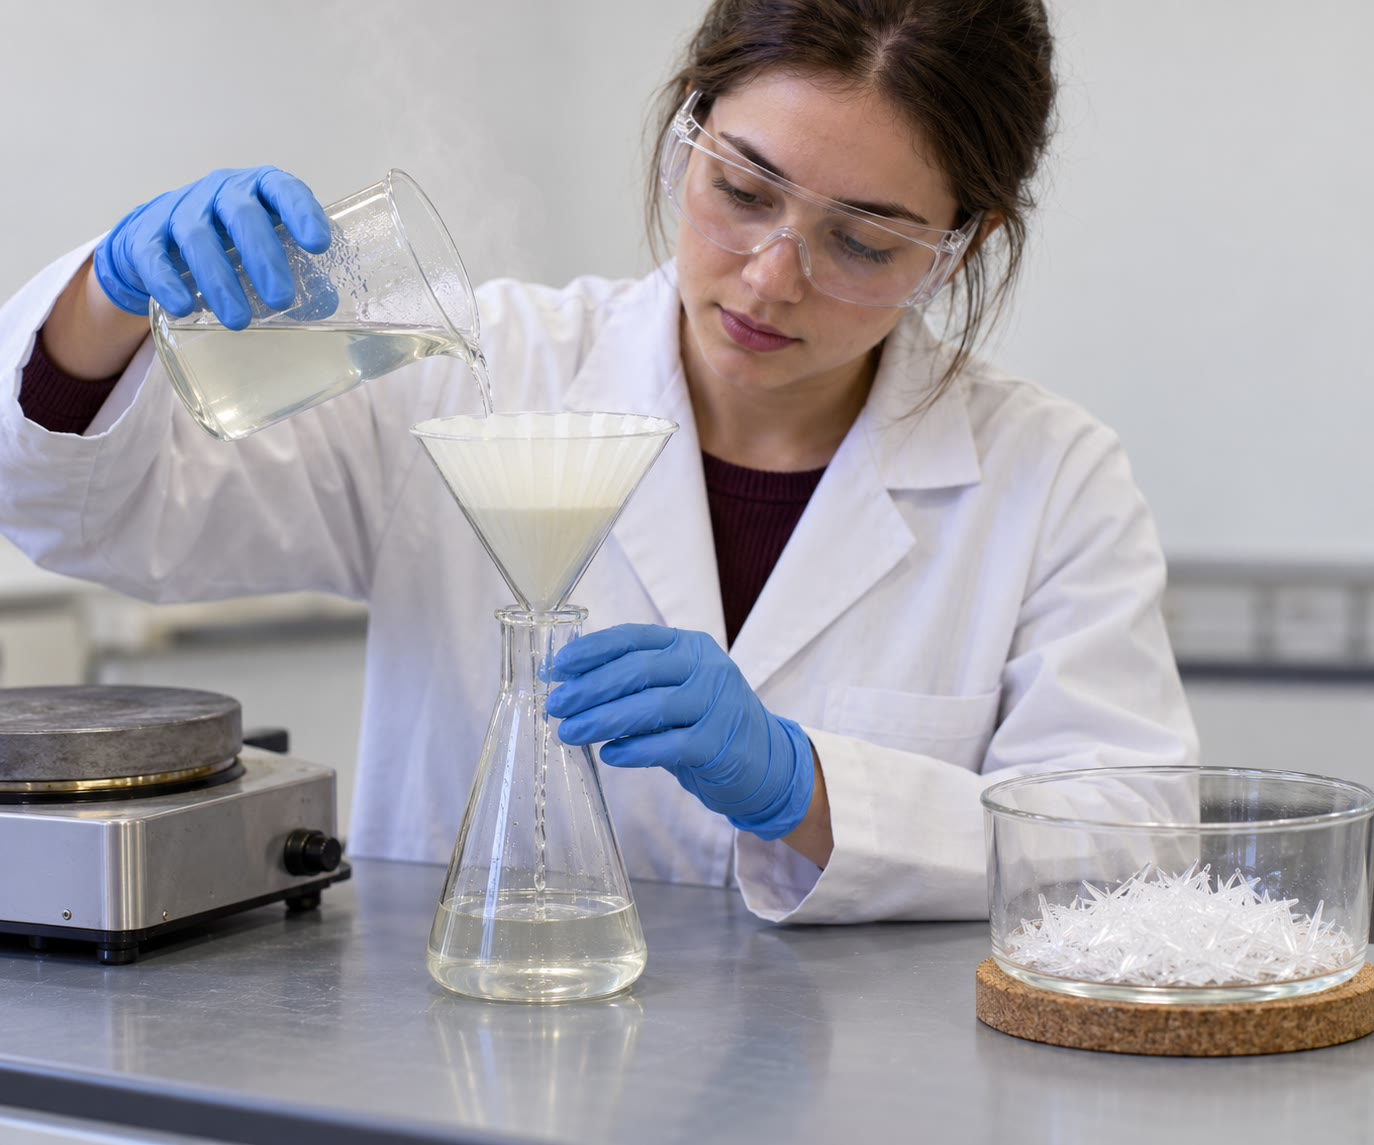
\includegraphics[width=0.5\linewidth]{images/book2/ai/b1-29-recrystallisation.jpg}

{\small Penyaringan panas selama \omterm{def:b1:lab-techniques-1:recrystallisation}{rekristalisasi}: kacamata pelindung,
sarung tangan, dan jas laboratorium; larutan panas melewati kertas saring
berlipat, yang menahan pengotor yang tidak larut. Jarum-jarum \omterm{def:b1:crystals-metals:crystal}{kristal}
produk hasil \omterm{def:b1:lab-techniques-1:recrystallisation}{rekristalisasi} menunggu di cawan sebelah kanan.}
\end{omfigure}

\section{Bahaya dan labelnya}

\begin{definition}[Bahaya dan risiko]\label{def:b1:lab-techniques-1:hazard}
\emph{Bahaya}\index{bahaya} adalah sifat intrinsik sebuah zat (atau
sebuah situasi) yang dapat menimbulkan kerugian: sifat mudah menyala,
sifat korosif, toksisitas. \emph{Risiko}\index{risiko} adalah
kemungkinan kerugian itu benar-benar terjadi, beserta tingkat
keparahannya, dalam kondisi penggunaan tertentu: risiko bergantung pada
bahaya dan pada paparan (jumlah, konsentrasi, lamanya, jalur masuk,
perlindungan).
\end{definition}

\omterm{def:b1:lab-techniques-1:hazard}{Bahaya} tidak dapat diubah tanpa mengubah zatnya; \omterm{def:b1:lab-techniques-1:hazard}{risiko} dikurangi dengan
mengendalikan paparan: jumlah yang lebih kecil, larutan yang lebih encer,
lemari asam, sarung tangan dan kacamata pelindung, atau pereaksi yang
kurang berbahaya untuk pekerjaan yang sama.

\begin{definition}[Pelabelan GHS]\label{def:b1:lab-techniques-1:ghs}
Label bahan kimia mengikuti Sistem Harmonisasi Global (GHS).
\begin{itemize}
  \item \emph{Piktogram bahaya}\index{piktogram bahaya} adalah simbol hitam
        di atas belah ketupat putih berbingkai merah; ada sembilan
        piktogram, \texttt{GHS01} sampai \texttt{GHS09}.
  \item \emph{Kata sinyal}\index{kata sinyal} adalah \emph{Bahaya} untuk
        kategori \omterm{def:b1:lab-techniques-1:hazard}{bahaya} yang lebih parah dan \emph{Peringatan} untuk yang
        kurang parah; sebuah label hanya memuat satu kata sinyal, yaitu
        yang lebih parah.
  \item \emph{Pernyataan bahaya}\index{pernyataan bahaya} adalah frasa
        baku, berkode H diikuti tiga angka, yang menguraikan sebuah \omterm{def:b1:lab-techniques-1:hazard}{bahaya}:
        H2xx untuk \omterm{def:b1:lab-techniques-1:hazard}{bahaya} fisik, H3xx untuk \omterm{def:b1:lab-techniques-1:hazard}{bahaya} kesehatan, dan H4xx
        untuk \omterm{def:b1:lab-techniques-1:hazard}{bahaya} lingkungan.
  \item \emph{Pernyataan kehati-hatian}\index{pernyataan kehati-hatian},
        berkode P dan tiga angka, memberikan tindakan yang harus diambil:
        P1xx untuk hal umum, P2xx untuk pencegahan, P3xx untuk tanggapan,
        P4xx untuk penyimpanan, dan P5xx untuk pembuangan.
  \item \emph{Lembar data keselamatan}\index{lembar data keselamatan}
        adalah dokumen yang diberikan pemasok bersama produknya, dalam
        bagian-bagian baku: identifikasi, \omterm{def:b1:lab-techniques-1:hazard}{bahaya}, komposisi, pertolongan
        pertama, pemadaman kebakaran, penanganan dan penyimpanan,
        pengendalian paparan dan perlindungan, sifat fisika dan kimia,
        kestabilan, toksisitas, pembuangan, dan pengangkutan.
\end{itemize}
\end{definition}

\begin{omfigure}
\setlength{\tabcolsep}{5pt}
\begin{tabular}{ccccc}
\begin{tabular}[t]{@{}c@{}}\ghs[1.25cm]{GHS01}\\[2pt]\footnotesize GHS01\\\footnotesize mudah meledak\end{tabular} &
\begin{tabular}[t]{@{}c@{}}\ghs[1.25cm]{GHS02}\\[2pt]\footnotesize GHS02\\\footnotesize mudah menyala\end{tabular} &
\begin{tabular}[t]{@{}c@{}}\ghs[1.25cm]{GHS03}\\[2pt]\footnotesize GHS03\\\footnotesize pengoksidasi\end{tabular} &
\begin{tabular}[t]{@{}c@{}}\ghs[1.25cm]{GHS04}\\[2pt]\footnotesize GHS04\\\footnotesize gas bertekanan\end{tabular} &
\begin{tabular}[t]{@{}c@{}}\ghs[1.25cm]{GHS05}\\[2pt]\footnotesize GHS05\\\footnotesize korosif\end{tabular} \\[8pt]
\begin{tabular}[t]{@{}c@{}}\ghs[1.25cm]{GHS06}\\[2pt]\footnotesize GHS06\\\footnotesize toksisitas akut\end{tabular} &
\begin{tabular}[t]{@{}c@{}}\ghs[1.25cm]{GHS07}\\[2pt]\footnotesize GHS07\\\footnotesize berbahaya, iritan\end{tabular} &
\begin{tabular}[t]{@{}c@{}}\ghs[1.25cm]{GHS08}\\[2pt]\footnotesize GHS08\\\footnotesize bahaya kesehatan\end{tabular} &
\begin{tabular}[t]{@{}c@{}}\ghs[1.25cm]{GHS09}\\[2pt]\footnotesize GHS09\\\footnotesize lingkungan\end{tabular} & \\
\end{tabular}

\smallskip
{\small Kesembilan piktogram GHS: bom meledak, nyala api, nyala api di
atas lingkaran, tabung gas, korosi, tengkorak dan tulang bersilang, tanda
seru, bahaya kesehatan (efek jangka panjang: kanker, mutasi, reproduksi,
sensitisasi saluran napas, aspirasi), dan lingkungan.}
% ledger: ghspic:GHS01, ghspic:GHS02, ghspic:GHS03, ghspic:GHS04,
% ghspic:GHS05, ghspic:GHS06, ghspic:GHS07, ghspic:GHS08, ghspic:GHS09
\end{omfigure}

\begin{example}[Membaca label etanol]
Sebotol etanol memuat piktogram GHS02 dan GHS07, \omterm{def:b1:lab-techniques-1:ghs}{kata sinyal}
\emph{Bahaya}, dan pernyataan H225 (cairan dan uap sangat mudah menyala,
sebuah \omterm{def:b1:lab-techniques-1:hazard}{bahaya} fisik, yang kategorinya menuntut \emph{Bahaya}) dan H319
(menyebabkan iritasi mata yang serius, sebuah \omterm{def:b1:lab-techniques-1:hazard}{bahaya} kesehatan, yang
dengan sendirinya cukup dengan \emph{Peringatan}). \omterm{def:b1:lab-techniques-1:ghs}{Pernyataan
kehati-hatiannya} antara lain P210 (jauhkan dari panas, percikan api, dan
nyala api terbuka; dilarang merokok), P233 (jaga wadah tetap tertutup
rapat), P280 (kenakan sarung tangan dan pelindung mata), P305+P351+P338
(jika terkena mata: bilas dengan hati-hati memakai air selama beberapa
menit, lepaskan lensa kontak, lanjutkan membilas), dan P403+P235 (simpan
di tempat yang berventilasi baik, jaga tetap sejuk). Akibat praktisnya:
tidak ada nyala api di meja kerja tempat etanol dipakai, kacamata
pelindung, botol yang tertutup.
\end{example}
% ledger: ghs:ethanol, hstat:H225, hstat:H319, pstat:P210, pstat:P233,
% pstat:P280, pstat:P305+P351+P338, pstat:P403+P235

\begin{method}[Mempersiapkan sesi praktikum dari lembar data keselamatan]\label{met:b1:lab-techniques-1:read-sds}
Untuk setiap zat yang dipakai atau terbentuk:
\begin{enumerate}
  \item bacalah piktogram, \omterm{def:b1:lab-techniques-1:ghs}{kata sinyal}, dan pernyataan H-nya (bagian 2
        lembar itu), dan catatlah \omterm{def:b1:lab-techniques-1:hazard}{bahaya} fisik (kebakaran, tekanan,
        reaktivitas) secara terpisah dari \omterm{def:b1:lab-techniques-1:hazard}{bahaya} kesehatan dan
        lingkungan;
  \item untuk setiap operasi (penimbangan, pemanasan, pemindahan,
        penyaringan), perkirakan paparannya: jumlah, wujud (cairan yang
        mudah menguap atau serbuk halus mencapai paru-paru), lamanya;
  \item pilihlah tindakannya: penggantian dengan pereaksi yang kurang
        berbahaya, skala yang lebih kecil, lemari asam, lalu alat
        pelindung diri (pernyataan P2xx);
  \item rencanakan tanggapan terhadap insiden (P3xx: mata, kulit,
        tertelan, kebakaran) dan ke mana setiap limbah dibuang (P5xx).
\end{enumerate}
\end{method}

\begin{inthelab}[Limbah]
Pada dasarnya tidak ada yang dibuang ke bak cuci. Pelarut organik
dikumpulkan dalam dua wadah, terhalogenasi (diklorometana, kloroform) dan
tidak terhalogenasi (etanol, propanon, sikloheksana, etil etanoat),
karena keduanya diolah secara berbeda; larutan asam dan basa berair
dinetralkan sebelum dibuang; larutan ion logam berat (kromium, tembaga,
perak) mempunyai wadahnya sendiri; pecahan kaca dan padatan yang
tercemar dipisahkan dari sampah biasa. Pernyataan P273, ``hindarkan
pelepasan ke lingkungan'', pada sebuah label mengingatkan bahwa wadah
limbah, bukan saluran pembuangan, adalah akhir dari percobaan.
% ledger: pstat:P273
\end{inthelab}

\section{Pengukuran dan ketidakpastian}

Nilai terukur tidak pernah sama persis dengan nilai besaran yang diukur:
ulangi pengukurannya, maka hasilnya sedikit berubah; bacalah skalanya,
maka angka terakhirnya adalah tebakan. Ketidakpastian menyatakan seberapa
jauh dari nilai terukur itu nilai sebenarnya secara wajar dapat terletak.

\begin{definition}[Ketidakpastian pengukuran]\label{def:b1:lab-techniques-1:uncertainty}
\begin{itemize}
  \item \emph{Ketidakpastian pengukuran}\index{ketidakpastian pengukuran}
        adalah parameter yang mencirikan sebaran nilai-nilai yang secara
        wajar dapat diberikan kepada besaran yang diukur.
  \item \emph{Ketidakpastian baku}\index{ketidakpastian baku} $u(x)$
        adalah ketidakpastian itu yang dinyatakan sebagai simpangan baku.
  \item \emph{Evaluasi tipe A}\index{evaluasi tipe A} memperoleh $u$
        melalui analisis statistik serangkaian pengukuran berulang;
        \emph{evaluasi tipe B}\index{evaluasi tipe B} memperolehnya dengan
        cara lain apa pun: skala sebuah instrumen, toleransi yang
        dinyatakan oleh pembuatnya, sertifikat kalibrasi, banyaknya angka
        sebuah nilai dalam tabel.
  \item \emph{Ketidakpastian diperluas}\index{ketidakpastian diperluas}
        $U = k\,u$ adalah ketidakpastian baku yang dikalikan dengan faktor
        cakupan $k$, biasanya $k = 2$; untuk distribusi normal, selang
        $x \pm 2u$ memuat nilai sebenarnya dengan peluang sekitar
        \qty{95}{\percent}.
  \item \emph{Ketidakpastian relatif}\index{ketidakpastian relatif}
        adalah $u(x)/|x|$, sering dinyatakan dalam persen.
\end{itemize}
\end{definition}

\begin{proposition}[Evaluasi tipe A]\label{prop:b1:lab-techniques-1:type-a}
Jika dilakukan $n$ pengukuran independen $x_1, \dots, x_n$ terhadap
besaran yang sama, taksiran terbaiknya adalah rata-ratanya $\bar x$;
simpangan baku eksperimennya adalah
\[
  s = \sqrt{\frac{1}{n-1} \sum_{i=1}^{n} (x_i - \bar x)^2},
\]
dan \omterm{def:b1:lab-techniques-1:uncertainty}{ketidakpastian baku} rata-ratanya adalah $u(\bar x) = s/\sqrt{n}$.
\end{proposition}
\begin{proof}[\omnameProof]
\emph{Diterima tanpa bukti pada tingkat ini}; statistika pengukuran
berulang, termasuk koefisien Student yang dipakai jika $n$ kecil, dibahas
dalam jilid Tahun 2.
\end{proof}

\begin{omfigure}
\begin{tikzpicture}
\begin{axis}[width=7.4cm, height=5cm, xlabel={volume titik akhir (\unit{mL})},
  ylabel={banyaknya pembacaan}, ymin=0, ymax=8.5, xmin=12.2, xmax=12.7,
  xtick={12.2,12.3,12.4,12.5,12.6,12.7},
  xticklabel style={/pgf/number format/fixed, /pgf/number format/precision=1},
  axis lines=left, every axis plot/.append style={line join=round}]
  \addplot[ybar, bar width=0.045, fill=omDef!35, draw=omDef!80!black]
    table[x=V, y=count] {figdata/out/bachelor-1-type-a-uncertainty-a.dat};
  \addplot[omThm, thick, smooth]
    table[x=V, y=g] {figdata/out/bachelor-1-type-a-uncertainty-b.dat};
  \draw[omProp, thick, <->] (axis cs:12.384,7.6) -- (axis cs:12.526,7.6);
  \node[omProp, font=\small, above] at (axis cs:12.455,7.6) {$\bar V \pm s$};
\end{axis}
\end{tikzpicture}\hspace{0.6cm}%
\begin{tikzpicture}
\begin{axis}[width=5.6cm, height=5cm, xlabel={$x - x_0$}, ylabel={kerapatan},
  ymin=0, ymax=0.8, xmin=-1.6, xmax=1.6, xtick={-1,0,1},
  xticklabels={$-a$, $0$, $a$}, ytick={0.5}, yticklabels={$\frac{1}{2a}$},
  axis lines=left]
  \addplot[omDef!80!black, thick, fill=omDef!25] coordinates
    {(-1,0) (-1,0.5) (1,0.5) (1,0)} \closedcycle;
  \draw[omProp, thick, <->] (axis cs:-0.577,0.62) -- (axis cs:0.577,0.62);
  \node[omProp, font=\small, above] at (axis cs:0,0.62) {$\pm a/\sqrt3$};
\end{axis}
\end{tikzpicture}

{\small Kiri: dua puluh pembacaan \omterm{def:b1:titration-methods:titration}{titik akhir} \omterm{def:b1:titration-methods:titration}{titrasi} yang sama (data
ilustratif), dibaca sampai \qty{0.05}{mL}, dengan kurva normal yang
rata-ratanya sama,
$\bar V = \qty{12.455}{mL}$, dan simpangan bakunya sama, $s = \qty{0.071}{mL}$.
Kanan: distribusi persegi panjang pada \omterm{def:b1:lab-techniques-1:uncertainty}{evaluasi tipe B}, untuk nilai yang
hanya diketahui terletak di antara $x_0 - a$ dan $x_0 + a$; simpangan
bakunya adalah
$a/\sqrt3$.}
\end{omfigure}

\begin{example}[Dua puluh titik akhir]
Untuk kedua puluh pembacaan pada gambar, $\bar V = \qty{12.455}{mL}$,
$s = \qty{0.071}{mL}$, dan $u(\bar V) = 0.071/\sqrt{20} = \qty{0.016}{mL}$.
Satu pembacaan mempunyai ketidakpastian sekitar $s$; rata-rata dua puluh
pembacaan sekitar
$s/\sqrt{20}$, empat setengah kali lebih kecil. Hasilnya adalah
$V = \qty{12.46}{mL}$ dengan $U = 2u = \qty{0.03}{mL}$.
\end{example}

\begin{proposition}[Evaluasi tipe B untuk distribusi persegi panjang]\label{prop:b1:lab-techniques-1:type-b}
Jika yang diketahui tentang sebuah besaran hanyalah bahwa besaran itu
terletak, dengan peluang yang sama, di mana saja di antara $x_0 - a$ dan
$x_0 + a$, \omterm{def:b1:lab-techniques-1:uncertainty}{ketidakpastian bakunya} adalah
\[
  u = \frac{a}{\sqrt3}.
\]
\end{proposition}
\begin{proof}
Kerapatan peluangnya adalah $1/(2a)$ pada $[x_0 - a, x_0 + a]$ dan nol di
tempat lain; rata-ratanya adalah $x_0$ karena simetri dan variansnya adalah
\[
  u^2 = \int_{x_0-a}^{x_0+a} (x - x_0)^2 \frac{\mathrm{d}x}{2a}
      = \frac{1}{2a} \left[\frac{t^3}{3}\right]_{-a}^{a}
      = \frac{1}{2a}\cdot\frac{2a^3}{3} = \frac{a^2}{3}. \qedhere
\]
\end{proof}

\begin{example}[Pembacaan dan toleransi]
Buret yang bergaris skala setiap \qty{0.1}{mL} dibaca sampai setengah
skala: pembacaannya terletak dalam $\pm\qty{0.05}{mL}$ dari nilai yang
dicatat, sehingga
$u = 0.05/\sqrt3 = \qty{0.029}{mL}$. Pipet \qty{20}{mL} yang pembuatnya
menyatakan toleransi $\pm\qty{0.03}{mL}$ mengeluarkan volumenya dengan
$u = 0.03/\sqrt3 = \qty{0.017}{mL}$. Nilai dalam tabel yang diberikan
sebagai \qty{135}{\celsius} diketahui sampai $\pm\qty{0.5}{\celsius}$: $u = \qty{0.29}{\celsius}$.
\end{example}

\begin{proposition}[Menggabungkan ketidakpastian]\label{prop:b1:lab-techniques-1:combine}
Untuk besaran-besaran yang independen: jika $y = x_1 + x_2$ atau $y = x_1 - x_2$, maka
$u(y)^2 = u(x_1)^2 + u(x_2)^2$; jika $y = x_1 x_2$ atau $y = x_1/x_2$, maka
\[
  \left(\frac{u(y)}{y}\right)^2 = \left(\frac{u(x_1)}{x_1}\right)^2
  + \left(\frac{u(x_2)}{x_2}\right)^2 .
\]
Beberapa sumber ketidakpastian pada besaran yang sama (sebuah bagian
tipe A dan bagian-bagian tipe B) digabungkan dengan cara yang sama,
sebagai jumlah kuadrat.
\end{proposition}
\admitted

Yang dijumlahkan adalah kuadratnya, bukan ketidakpastian itu sendiri: dua
galat yang independen jarang mendorong ke arah yang sama dengan ukuran
penuh. Volume \omterm{def:b1:titration-methods:titration}{titrasi} adalah selisih dua pembacaan buret, sehingga
ketidakpastian pembacaannya adalah
$\sqrt2 \times \qty{0.029}{mL} = \qty{0.041}{mL}$; dan satu sumber
ketidakpastian yang besar mendominasi sumber-sumber lainnya, dan di
situlah perbaikan seharusnya dicari. Aturan umumnya, dengan turunan
parsial, termasuk dalam jilid Tahun 2.

\begin{method}[Melaporkan hasil]\label{met:b1:lab-techniques-1:report-result}
\begin{enumerate}
  \item Daftarlah sumber-sumber ketidakpastian; evaluasilah masing-masing
        sebagai \omterm{def:b1:lab-techniques-1:uncertainty}{ketidakpastian baku} (tipe A dari sebuah deret, tipe B
        sebagai $a/\sqrt3$ dari setengah lebar).
  \item Gabungkan semuanya sebagai jumlah kuadrat (\cref{prop:b1:lab-techniques-1:combine}).
  \item Berikan \omterm{def:b1:lab-techniques-1:uncertainty}{ketidakpastian diperluas} $U = 2u$ dengan satu atau dua
        angka penting, dan bulatkan nilainya sampai tempat desimal yang
        sama: $x = (\text{nilai} \pm U)$ satuan, $k = 2$.
\end{enumerate}
\end{method}

\begin{definition}[Deviasi ternormalisasi]\label{def:b1:lab-techniques-1:z-score}
\emph{Deviasi ternormalisasi}\index{deviasi ternormalisasi} (atau skor $z$)
antara dua nilai independen $x_1$ dan $x_2$ dari besaran yang sama,
dengan \omterm{def:b1:lab-techniques-1:uncertainty}{ketidakpastian baku} $u_1$ dan $u_2$, adalah
\[
  z = \frac{|x_1 - x_2|}{\sqrt{u_1^2 + u_2^2}} .
\]
Kedua nilai itu dikatakan kompatibel jika $z \le 2$; nilai terukur
kompatibel dengan nilai acuan dengan syarat yang sama.
\end{definition}

\begin{example}[Kedua mahasiswa]
Kedua titik leleh pada pembukaan bab, \qty{134}{\celsius} dan
\qty{136}{\celsius}, masing-masing diperoleh dengan \omterm{def:b1:lab-techniques-1:uncertainty}{ketidakpastian baku}
\qty{0.8}{\celsius} (pembacaan dan kalibrasi bangku pemanas). Maka
$z = 2/\sqrt{0.8^2 + 0.8^2} = 1.8 \le 2$: kedua mahasiswa itu sepakat.
Rata-ratanya,
\qty{135}{\celsius}, juga kompatibel dengan titik leleh aspirin dalam
tabel, \qty{135}{\celsius} pada pemanasan cepat. Nilai dalam tabel yang
diberikan sampai satuan mempunyai $u = 0.5/\sqrt3 = \qty{0.29}{\celsius}$, sehingga satu
pembacaan dengan $u = \qty{0.8}{\celsius}$ kompatibel dengannya selama
pembacaan itu terletak dalam
$2\sqrt{0.8^2 + 0.29^2} = \qty{1.7}{\celsius}$ darinya: pembacaan di
bawah sekitar \qty{133}{\celsius} akan menunjukkan produk yang tidak
murni.
\end{example}
% ledger: mp:aspirin

\section{Pemisahan}

\begin{definition}[Koefisien partisi]\label{def:b1:lab-techniques-1:partition-coefficient}
Jika sebuah zat terlarut A terbagi, pada kesetimbangan, di antara dua
pelarut yang tidak \omterm{def:b1:intermolecular-forces-solvents:miscibility}{dapat bercampur}, sebuah \omterm{def:b1:extent-q-and-k:system}{fase} organik dan sebuah \omterm{def:b1:extent-q-and-k:system}{fase}
berair, perbandingan konsentrasinya
\[
  K = \frac{[\mathrm{A}]_{\mathrm{org}}}{[\mathrm{A}]_{\mathrm{aq}}}
\]
adalah, untuk larutan encer pada suhu tertentu, sebuah tetapan:
\emph{koefisien partisi}\index{koefisien partisi} A di antara kedua
pelarut itu.
\end{definition}

\begin{proposition}[Beberapa kali ekstraksi lebih baik daripada sekali]\label{prop:b1:lab-techniques-1:multiple-extractions}
Volume $V_a$ larutan berair diekstraksi $n$ kali, setiap kali dengan
volume $V_o$ pelarut organik yang baru. Fraksi A yang tersisa dalam \omterm{def:b1:extent-q-and-k:system}{fase}
berair adalah
\[
  f_n = \left(1 + K \frac{V_o}{V_a}\right)^{-n}.
\]
Untuk volume total pelarut yang tetap, $n$ porsi kecil mengekstraksi
lebih banyak daripada satu porsi besar.
\end{proposition}
\begin{proof}
Misalkan $m$ adalah jumlah A dalam \omterm{def:b1:extent-q-and-k:system}{fase} berair sebelum sebuah ekstraksi,
dan
$m'$ sesudahnya. Pada kesetimbangan, \omterm{def:b1:extent-q-and-k:system}{fase} organik memuat $m - m'$, dan
$K = \dfrac{(m - m')/V_o}{m'/V_a}$, sehingga $m - m' = K\dfrac{V_o}{V_a} m'$ dan
$m' = m\big/\bigl(1 + K V_o/V_a\bigr)$. Setiap ekstraksi mengalikan
jumlah yang tersisa dengan faktor yang sama; sesudah $n$ ekstraksi, $f_n$
adalah pangkat ke-$n$. Dengan volume total $V$ yang dibagi menjadi $n$
porsi $V/n$,
$\ln f_n = -n \ln(1 + KV/(nV_a))$; karena $\ln(1+t)/t$ menurun terhadap $t$,
$n \ln(1 + t/n)$ naik terhadap $n$ untuk $t = KV/V_a > 0$, dan $f_n$
menurun, menuju limit $\mathrm{e}^{-KV/V_a}$.
\end{proof}

\begin{example}[Satu porsi atau tiga]
Sebuah zat terlarut dengan $K = 4$ diekstraksi dari \qty{100}{mL} air
dengan \qty{60}{mL} etil etanoat. Dalam satu porsi,
$f_1 = 1/(1 + 4 \times 0.6) = 0.29$: \qty{71}{\percent} terekstraksi.
Dalam tiga porsi masing-masing \qty{20}{mL}, $f_3 = (1 + 4 \times 0.2)^{-3} = 0.17$:
\qty{83}{\percent}. Etil etanoat ($\rho = \qty{0.90}{g/cm^3}$) menjadi
lapisan atas dalam corong pisah; diklorometana
($\rho = \qty{1.33}{g/cm^3}$) akan menjadi lapisan bawah.
\end{example}
% ledger: rho:ethyl-acetate, rho:CH2Cl2, rho:water

Penyaringan memisahkan padatan dari cairan. Dengan gravitasi, melalui
kertas saring berlipat dalam corong, penyaringan menahan pengotor yang
tidak larut dari larutan panas yang tidak boleh mendingin di perjalanan
(penyaringan panas, seperti pada foto di awal bab). Dengan tekanan
rendah, dalam corong Büchner di atas labu isap (seperti yang digambar
dalam jilid sekolah), penyaringan mengumpulkan padatan dengan cepat dan
meninggalkannya hampir kering; padatan itu dicuci di atas penyaring
dengan sedikit pelarut dingin.

\begin{definition}[Rekristalisasi]\label{def:b1:lab-techniques-1:recrystallisation}
\emph{Rekristalisasi}\index{rekristalisasi} memurnikan padatan dengan
melarutkannya dalam pelarut panas sesedikit mungkin, yaitu pelarut yang
melarutkannya dengan sangat baik dalam keadaan panas dan sedikit dalam
keadaan dingin, lalu membiarkannya mengkristal ketika didinginkan;
pengotor tetap terlarut dalam pelarut dingin (cairan induk) atau, jika
tidak larut, dihilangkan lebih dahulu melalui penyaringan panas.
\end{definition}

\begin{method}[Merekristalisasi padatan]\label{met:b1:lab-techniques-1:recrystallise}
\begin{enumerate}
  \item Pilihlah pelarutnya: produk sangat larut dalam keadaan panas dan
        sedikit larut dalam keadaan dingin, pengotor yang larut tetap
        larut walaupun dingin, tidak bereaksi dengan produk, titik didih
        di bawah titik leleh produk; campuran dua pelarut yang \omterm{def:b1:intermolecular-forces-solvents:miscibility}{dapat
        bercampur} (etanol dan air) dapat disesuaikan dengan produknya.
  \item Larutkan padatan kasar dalam pelarut mendidih sesedikit mungkin,
        yang ditambahkan sedikit demi sedikit, di bawah refluks jika
        pelarutnya mudah menguap atau mudah menyala.
  \item Jika masih ada pengotor yang tidak larut, saringlah selagi panas.
  \item Biarkan larutan mendingin perlahan, lalu dalam es: pendinginan
        yang lambat menghasilkan \omterm{def:b1:crystals-metals:crystal}{kristal} yang lebih besar dan lebih
        murni, yang memerangkap lebih sedikit cairan induk.
  \item Saringlah dengan tekanan rendah, cucilah dengan sedikit pelarut
        sedingin es, keringkan, timbanglah; periksalah kemurniannya
        (titik leleh, KLT).
\end{enumerate}
\end{method}

\begin{example}[Harga kemurnian]
Aspirin larut dalam air sekitar \qty{3.3}{g/L} pada \qty{25}{\celsius}
dan \qty{10}{g/L} pada \qty{37}{\celsius}, dan jauh lebih banyak di dekat
titik didih. Jika \qty{40}{mL} cairan induk dan \qty{10}{mL} air pencuci
meninggalkan penyaring pada \qty{25}{\celsius}, keduanya membawa pergi
sekitar
$\qty{0.050}{L} \times \qty{3.3}{g/L} = \qty{0.17}{g}$ aspirin, berapa pun
kemurniannya. Setiap mililiter pelarut di atas jumlah minimum mengurangi
\omterm{def:b1:extent-q-and-k:fractional-extent}{rendemen}.
\end{example}
% ledger: sol:aspirin-25, sol:aspirin-37

Sebuah cairan dimurnikan, atau dua cairan yang titik didihnya berjauhan
dipisahkan, melalui \emph{distilasi sederhana}: campurannya dididihkan,
uapnya, yang lebih kaya akan komponen yang lebih mudah menguap,
diembunkan dan dikumpulkan. Suhu pada lengan samping adalah suhu uap yang
terdistilasi; selama suhu itu tetap, sebuah zat murni sedang melintas.
Cairan yang titik didihnya berdekatan memerlukan distilasi fraksional,
dengan sebuah kolom di antara labu dan kepala distilasi, yang dibahas
bersama diagram cair--uap dalam jilid Tahun 2.

\begin{omfigure}
\begin{tikzpicture}[font=\small, scale=0.95]
  \pic[transform shape] at (0,0) {heatingmantle};
  \pic[transform shape] at (0,0) {rbflask={0.45}{orange!25}};
  \foreach \x/\y in {-0.35/0.25,0.05/0.18,0.35/0.3}
    \fill[black!55] (\x,\y) circle (0.06);
  \pic[transform shape] (s) at (0,3.0) {stillhead};
  \pic[transform shape] at ($(s-top)+(0,-0.75)$) {thermometer};
  \pic[transform shape, rotate=-20] (c) at (s-arm) {liebig={3.4}};
  \coordinate (cend) at ($(s-arm)+(-20:3.4)$);
  \pic[transform shape] (a) at (cend) {adapter};
  \pic[transform shape] at ($(a-tip)+(0,-2.4)$) {erlenmeyer={0.22}{orange!12}};
  \draw[<-, omProp, thick] (0.12,3.72) -- (-1.4,4.4) node[left, text=black,
    align=right] {bola termometer\\ sejajar dengan lengan samping};
  \draw[<-, omProp, thick] ($(s-arm)+(-20:0.65)+(0.65,0.65)$) -- ++(0.2,0.9)
    node[above, text=black] {air keluar};
  \draw[<-, omProp, thick] ($(s-arm)+(-20:2.7)+(-0.2,-0.6)$) -- ++(0.05,-0.9)
    node[below, text=black] {air masuk};
  \draw[<-, omProp, thick] (-0.3,0.27) -- (-2.2,0.7) node[left, text=black]
    {batu didih};
  \draw[<-, omProp, thick] (1.35,-0.6) -- (2.3,-1.1) node[right, text=black]
    {mantel pemanas};
  \draw[<-, omProp, thick] ($(a-tip)+(0.75,-2.0)$) -- ++(1.0,0.2)
    node[right, text=black] {distilat};
\end{tikzpicture}

{\small Distilasi sederhana. Termometer membaca suhu uap yang memasuki
kondensor; air pendingin masuk di ujung bawah kondensor agar mantelnya
tetap penuh; batu didih mencegah letupan didih yang hebat; alat itu
terbuka ke udara pada penampung.}
\end{omfigure}

\begin{safety}{\ghs[5mm]{GHS02}}
Alat distilasi tidak pernah tertutup: jika dipanaskan, sistem yang
tertutup rapat akan pecah. Batu didih ditambahkan ke dalam cairan yang
dingin, tidak pernah ke dalam cairan yang sudah panas (cairan itu dapat
langsung meluap). Distilat yang mudah menyala dikumpulkan jauh dari nyala
api, dengan penampung yang bila perlu diletakkan dalam es.
\end{safety}

\section{Identifikasi dan pemeriksaan kemurnian}

\begin{definition}[Faktor retensi]\label{def:b1:lab-techniques-1:retention-factor}
Dalam kromatografi lapis tipis (KLT), setitik sampel diteteskan pada
garis awal di dekat kaki sebuah pelat yang dilapisi \omterm{def:b1:extent-q-and-k:system}{fase} diam (silika);
pelat itu berdiri di dalam bejana tertutup berisi sedikit eluen, yang
naik melalui lapisan itu secara kapiler dan membawa spesi-spesi dengan
laju yang berbeda. \emph{Faktor retensi}\index{faktor retensi} sebuah
spesi adalah
\[
  R_f = \frac{\text{jarak yang ditempuh noda}}
             {\text{jarak yang ditempuh garis depan eluen}},
\]
keduanya diukur dari garis awal; $0 \le R_f \le 1$, dan untuk \omterm{def:b1:extent-q-and-k:system}{fase} diam,
eluen, dan suhu tertentu, faktor retensi mencirikan spesi itu.
\end{definition}

Pada silika yang polar, spesi polar ditahan lebih kuat daripada spesi
yang kurang polar dan mempunyai $R_f$ yang lebih kecil; eluen yang lebih
polar menggerakkan setiap noda lebih jauh. Dua spesi dengan $R_f$ yang
sama pada satu pelat mungkin tetap berbeda; dua $R_f$ yang berbeda
membuktikan bahwa keduanya berbeda. Produk yang murni memberikan satu
noda.

\begin{omfigure}
\begin{tikzpicture}[font=\small, scale=1.7]
  \pic[transform shape] at (0,0) {tlcplate};
  \draw[omDef!80!black, densely dashed, line width=0.5pt] (-0.7,2.7) -- (0.7,2.7);
  \foreach \x in {-0.4,0,0.4} \fill[black!60] (\x,0.4) circle (0.025);
  \fill[omThm!70] (-0.4,{0.4+0.30*2.3}) ellipse (0.09 and 0.06);
  \fill[omDef!70] (0,{0.4+0.65*2.3}) ellipse (0.09 and 0.06);
  \fill[omThm!70] (0.4,{0.4+0.30*2.3}) ellipse (0.09 and 0.06);
  \fill[omDef!70] (0.4,{0.4+0.65*2.3}) ellipse (0.09 and 0.06);
  \node[below] at (-0.4,0) {A}; \node[below] at (0,0) {B};
  \node[below] at (0.4,0) {M};
  \draw[omProp, thick, |<->|] (0.95,0.4) -- (0.95,{0.4+0.65*2.3})
    node[midway, right] {$d_{\mathrm{B}}$};
  \draw[omProp, thick, |<->|] (1.55,0.4) -- (1.55,2.7)
    node[midway, right] {$d_{\mathrm{depan}}$};
  \draw[omProp, thick, |<->|] (-0.95,0.4) -- (-0.95,{0.4+0.30*2.3})
    node[midway, left] {$d_{\mathrm{A}}$};
  \node[right, align=left, font=\footnotesize] at (0.75,2.85) {garis depan eluen};
  \draw[omProp, thick, <-] (-0.6,0.4) -- (-1.2,0.05) node[left, text=black, font=\footnotesize] {garis awal};
\end{tikzpicture}

{\small Pelat KLT yang telah dikembangkan: pembanding A dan B serta
campuran M, yang diteteskan pada garis awal. $R_f(\mathrm{A}) = d_{\mathrm{A}}/d_{\mathrm{depan}}
= 0.30$, $R_f(\mathrm{B}) = 0.65$; campuran itu memperlihatkan kedua noda,
pada ketinggian yang sama.}
\end{omfigure}

\begin{method}[Menjalankan KLT]\label{met:b1:lab-techniques-1:tlc}
\begin{enumerate}
  \item Gambarlah garis awal dengan pensil sekitar \qty{1}{cm} dari kaki
        pelat; teteskan noda-noda kecil larutan encer sampel dan
        pembanding bersebelahan.
  \item Tuangkan eluen setinggi beberapa milimeter ke dalam bejana (di
        bawah garis awal), tutuplah, biarkan atmosfernya jenuh; letakkan
        pelat di dalamnya.
  \item Angkat pelat ketika garis depan berada sekitar \qty{1}{cm} dari
        puncaknya; segera tandai garis depan itu; keringkan.
  \item Tampakkan noda-noda yang tidak berwarna (lampu ultraviolet pada
        pelat berfluoresensi, uap iodin, sebuah pewarna); lingkari dengan
        pensil.
  \item Ukurlah jaraknya dari garis awal dan hitunglah setiap $R_f$;
        bandingkan sampel dengan pembanding pada pelat yang sama.
\end{enumerate}
\end{method}

\begin{omfigure}
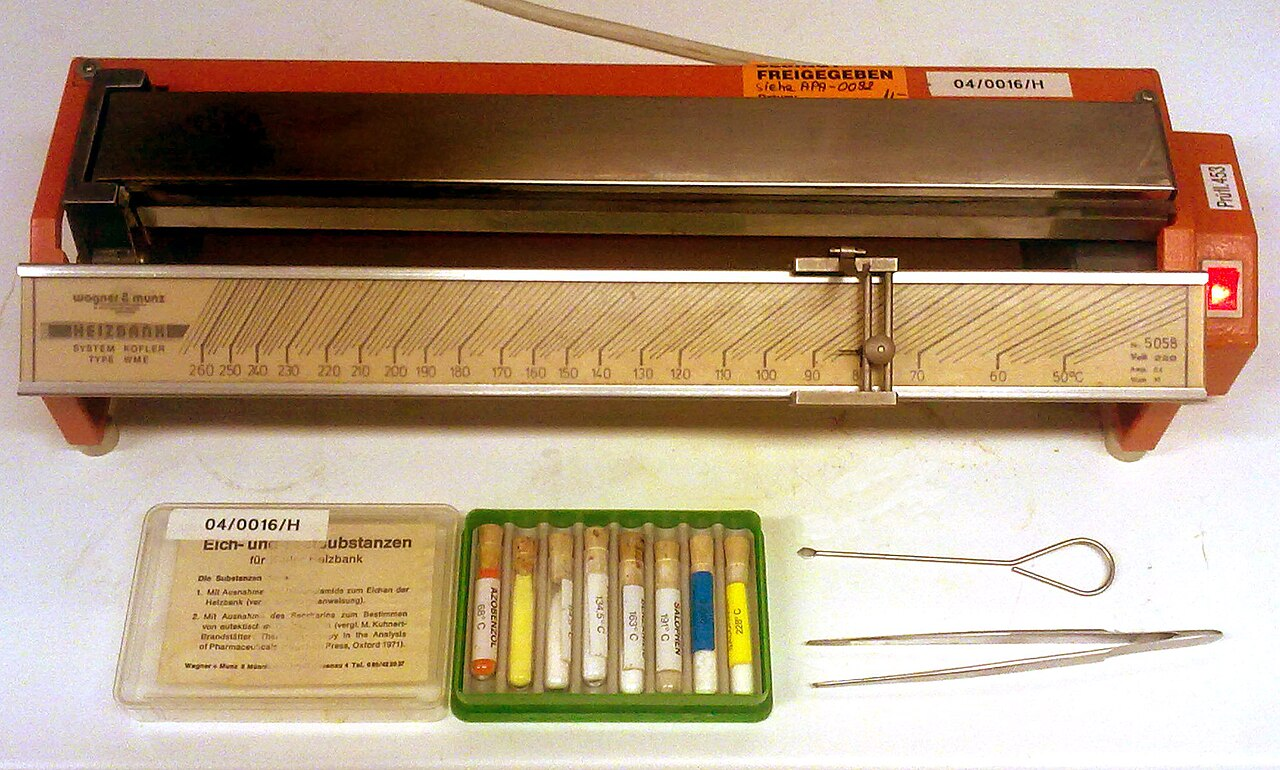
\includegraphics[width=0.62\linewidth]{images/book2/kofler-bench.jpg}

{\small Bangku pemanas (bangku Kofler): sebuah lempeng logam yang
dipanaskan pada salah satu ujungnya, dengan gradien suhu di sepanjangnya;
padatan, yang ditaburkan di atas lempeng itu, meleleh setelah melewati
sebuah garis yang tajam, yang dibaca pada skala dengan penunjuk. Kotak
itu berisi zat pembanding yang titik lelehnya diketahui, yang dipakai
untuk mengkalibrasinya. Foto: HBR, CC BY-SA 3.0, Wikimedia Commons.}
\end{omfigure}

\begin{method}[Mengukur titik leleh pada bangku pemanas]\label{met:b1:lab-techniques-1:melting-point}
\begin{enumerate}
  \item Nyalakan bangku pemanas jauh sebelumnya: gradiennya memerlukan
        waktu untuk menjadi mantap.
  \item Kalibrasilah bangku itu dengan zat pembanding murni yang meleleh
        dekat dengan nilai yang diharapkan, yang ditaburkan di atas
        lempeng; aturlah penunjuk sehingga skala membaca titik lelehnya
        pada garis itu.
  \item Taburkan beberapa \omterm{def:b1:crystals-metals:crystal}{kristal} sampel yang kering dari ujung dingin ke
        arah ujung panas; dorong \omterm{def:b1:crystals-metals:crystal}{kristal-kristal} itu maju mundur dengan
        spatula dan letakkan penunjuk pada batas yang di atasnya padatan
        langsung meleleh.
  \item Bacalah, ulangi, bersihkan lempengnya; ambillah rata-rata
        pembacaannya dan nyatakan ketidakpastiannya
        (\cref{met:b1:lab-techniques-1:report-result}).
\end{enumerate}
\end{method}

Zat kristalin yang murni meleleh dengan tajam pada titik lelehnya; zat
yang tidak murni mulai meleleh pada suhu yang lebih rendah dan meleleh
dalam suatu rentang suhu, karena pengotor menurunkan suhu tempat padatan
dan cairan berada bersama (alasannya, yaitu potensial kimia pelarut yang
diturunkan oleh zat terlarut, terdapat dalam jilid Tahun 2). Karena itu,
titik leleh yang jauh di bawah nilai dalam tabel, atau rentang leleh yang
lebar, mengungkapkan adanya pengotor; nilai yang kompatibel dengan nilai
dalam tabel, dalam arti \omterm{def:b1:lab-techniques-1:z-score}{deviasi ternormalisasi}, mendukung kemurnian tanpa
membuktikannya.

\begin{inthelab}[Mengkalibrasi bangku pemanas]
Zat pembanding dipilih sehingga mengapit nilai yang diharapkan.
Asetanilida, yang meleleh pada \qty{114.3}{\celsius}, dan asam benzoat,
pada \qty{122.4}{\celsius}, adalah standar klasik untuk produk yang
meleleh di antara \qty{110}{\celsius} dan \qty{130}{\celsius}; untuk
aspirin, standar di dekat \qty{135}{\celsius} lebih baik lagi. Aspirin
sendiri terurai ketika meleleh, sehingga titik leleh yang teramati
bergantung pada kecepatan pemanasannya: tabel memberikan
\qty{135}{\celsius} untuk pemanasan cepat, seperti yang dilakukan bangku
pemanas.
% ledger: mp:acetanilide, mp:benzoic, mp:aspirin
\end{inthelab}

Sebuah cairan diidentifikasi, dan kemurniannya diperiksa, melalui
\emph{indeks bias} $n_D$-nya, yaitu perbandingan kelajuan cahaya dalam
vakum dengan kelajuannya dalam cairan itu, yang diukur dengan garis D
kuning natrium pada suhu yang dinyatakan (biasanya \qty{20}{\celsius}),
sampai empat tempat desimal. Air mempunyai
$n_D = 1.333$, etanol 1.3611, dan sikloheksana 1.4266 pada \qty{20}{\celsius}.
Indeks itu sedikit menurun ketika suhu naik, sehingga instrumennya
dilengkapi termostat.
% ledger: nD:water, nD:ethanol, nD:cyclohexane

\begin{omfigure}
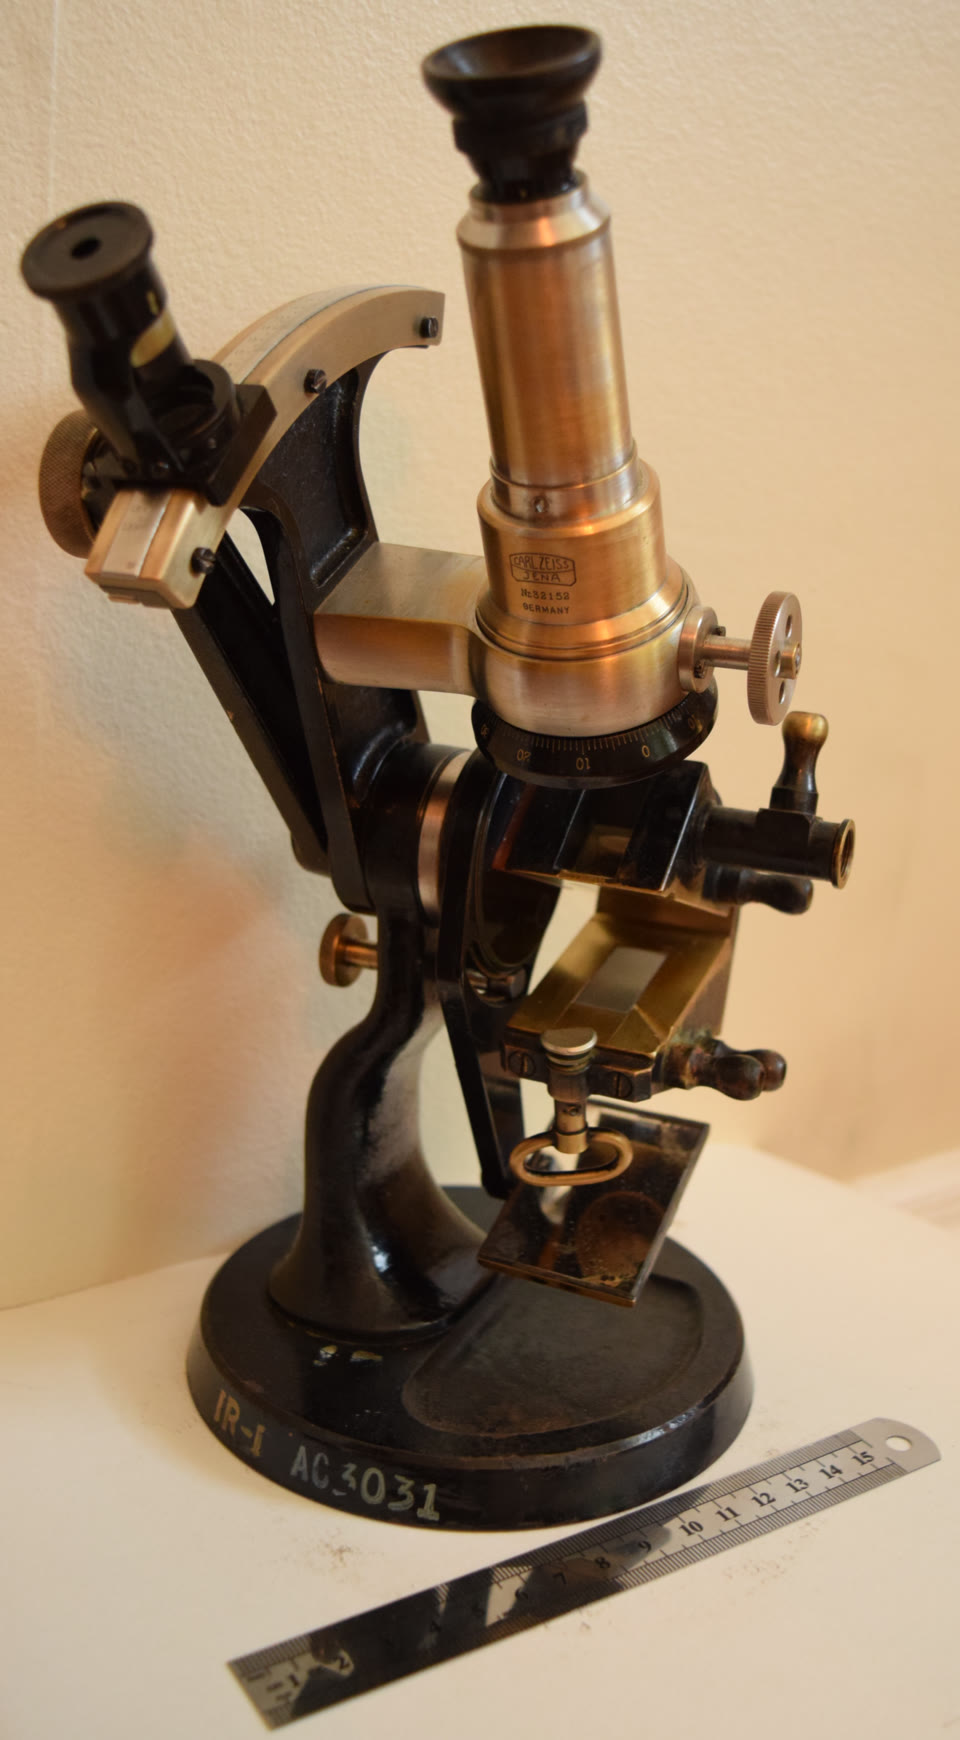
\includegraphics[height=6cm]{images/book2/abbe-refractometer.jpg}

{\small Refraktometer Abbe: setetes cairan diratakan di antara dua prisma;
lensa okuler memperlihatkan medan yang separuh terang dan separuh gelap,
dan batasnya, yang diimpitkan dengan benang silang, memberikan indeks
bias pada skala. Foto: Foreade, CC BY-SA 4.0, Wikimedia Commons.}
\end{omfigure}

\section{Latihan}

\begin{exercise}[$\star$]\label{exo:b1:lab-techniques-1:1}
Sebotol propanon memuat piktogram GHS02 dan GHS07 serta pernyataan H225,
H319, dan H336. \omterm{def:b1:lab-techniques-1:ghs}{Kata sinyal} apakah yang dimuatnya? Pernyataan manakah
yang menguraikan \omterm{def:b1:lab-techniques-1:hazard}{bahaya} fisik, dan manakah yang menguraikan \omterm{def:b1:lab-techniques-1:hazard}{bahaya}
kesehatan? Sebutkan dua tindakan pencegahan yang dituntutnya.
\end{exercise}

\begin{exercise}[$\star$]\label{exo:b1:lab-techniques-1:2}
\omterm{def:b1:lab-techniques-1:hazard}{Bahaya} atau \omterm{def:b1:lab-techniques-1:hazard}{risiko}? (a) Asam sulfat pekat menyebabkan luka bakar parah.
(b) Menimbang \qty{50}{mg} serbuk beracun di dalam lemari asam dengan
sarung tangan hanya sedikit memaparkan operatornya. (c) Natrium
melepaskan hidrogen dengan air. (d) Pelarut yang sama lebih berbahaya
jika dipakai panas dalam gelas kimia terbuka daripada dingin dalam botol
tertutup.
\end{exercise}

\begin{exercise}[$\star$]\label{exo:b1:lab-techniques-1:3}
Pada sebuah pelat KLT, garis depan eluen berada \qty{6.0}{cm} di atas
garis awal; sampel memberikan noda pada \qty{2.1}{cm} dan
\qty{4.2}{cm}. Hitunglah
$R_f$-nya. Sebuah pembanding yang diteteskan pada pelat yang sama naik
sampai \qty{4.2}{cm}: apa yang dapat dan tidak dapat disimpulkan?
\end{exercise}

\begin{exercise}[$\star$]\label{exo:b1:lab-techniques-1:4}
Buret yang bergaris skala setiap \qty{0.1}{mL} dibaca sampai setengah
skala. Hitunglah \omterm{def:b1:lab-techniques-1:uncertainty}{ketidakpastian baku} satu pembacaan, lalu \omterm{def:b1:lab-techniques-1:uncertainty}{ketidakpastian
baku} volume yang dikeluarkan, yaitu selisih dua pembacaan.
\end{exercise}

\begin{exercise}[$\star\star$]\label{exo:b1:lab-techniques-1:5}
Lima kali penimbangan sampel yang sama memberikan \qty{0.2512}{g},
\qty{0.2508}{g}, \qty{0.2515}{g}, \qty{0.2510}{g}, dan \qty{0.2505}{g}.
Hitunglah rata-ratanya, simpangan baku eksperimennya, \omterm{def:b1:lab-techniques-1:uncertainty}{ketidakpastian
baku} rata-ratanya, dan laporkan hasilnya dengan $k = 2$.
\end{exercise}

\begin{exercise}[$\star\star$]\label{exo:b1:lab-techniques-1:6}
Sebuah zat terlarut dengan \omterm{def:b1:lab-techniques-1:partition-coefficient}{koefisien partisi} $K = 3$ antara sebuah
pelarut organik dan air diekstraksi dari \qty{50}{mL} air dengan total
\qty{30}{mL} pelarut. Hitunglah fraksi yang terekstraksi dalam satu porsi,
dalam dua porsi masing-masing \qty{15}{mL}, dan dalam tiga porsi
masing-masing \qty{10}{mL}.
\end{exercise}

\begin{exercise}[$\star\star$]\label{exo:b1:lab-techniques-1:7}
Sebuah \omterm{def:b1:titration-methods:titration}{titrasi} memberikan konsentrasi \qty{0.1012}{mol/L} dengan
\omterm{def:b1:lab-techniques-1:uncertainty}{ketidakpastian baku} \qty{0.0006}{mol/L}; larutan itu dibuat pada
\qty{0.1000}{mol/L} dengan \omterm{def:b1:lab-techniques-1:uncertainty}{ketidakpastian baku} \qty{0.0002}{mol/L}.
Apakah kedua nilai itu kompatibel? Bagaimana jika ketidakpastian
\omterm{def:b1:titration-methods:titration}{titrasinya} \qty{0.0004}{mol/L}?
\end{exercise}

\begin{exercise}[$\star\star$]\label{exo:b1:lab-techniques-1:8}
\omterm{def:b1:precipitation:solubility}{Kelarutan} (nilai ilustratif, \unit{g} per \qty{100}{mL}) sebuah padatan
dalam tiga pelarut adalah: pelarut P, 1.5 dalam keadaan dingin dan 2.0
dalam keadaan mendidih; pelarut Q, 0.3 dingin dan 12 mendidih; pelarut R,
9 dingin dan 25 mendidih. Pelarut manakah yang cocok untuk \omterm{def:b1:lab-techniques-1:recrystallisation}{rekristalisasi},
dan mengapa bukan kedua pelarut lainnya? Dengan pelarut yang tepat,
berapa fraksi terbesar dari \qty{5.0}{g} padatan itu yang dapat diperoleh
kembali, jika dipakai pelarut mendidih sesedikit mungkin dan campurannya
didinginkan?
\end{exercise}

\begin{exercise}[$\star\star$]\label{exo:b1:lab-techniques-1:9}
Sebuah cairan tak berwarna, yang dijaga pada \qty{20}{\celsius}, mempunyai
$n_D = 1.3612$. Manakah di antara air, etanol, dan sikloheksana yang
mungkin merupakan cairan itu? Mengapa suhunya dinyatakan? Apa yang
ditunjukkan oleh nilai 1.350?
\end{exercise}

\begin{exercise}[$\star\star\star$]\label{exo:b1:lab-techniques-1:10}
Dengan data \cref{exo:b1:lab-techniques-1:6}, tunjukkan bahwa betapa pun
halusnya \qty{30}{mL} pelarut itu dibagi, paling banyak fraksi
$1 - \mathrm{e}^{-KV/V_a}$ zat terlarut yang dapat diekstraksi, dan
hitunglah fraksi itu. Berapa porsi yang diperlukan untuk mencapai
\qty{99}{\percent} dari limit itu?
\end{exercise}

\begin{exercise}[$\star\star\star$]\label{exo:b1:lab-techniques-1:11}
Sebuah besaran diketahui terletak di antara $x_0 - a$ dan $x_0 + a$,
dengan nilai di dekat
$x_0$ lebih mungkin: kerapatannya berbentuk segitiga, $(a - |x - x_0|)/a^2$.
Periksalah bahwa kerapatan itu ternormalisasi dan tunjukkan bahwa
\omterm{def:b1:lab-techniques-1:uncertainty}{ketidakpastian bakunya} adalah
$a/\sqrt6$. Bandingkan dengan kasus persegi panjang.
\end{exercise}

\begin{exercise}[$\star\star\star$]\label{exo:b1:lab-techniques-1:12}
Sebuah larutan baku dibuat dengan melarutkan sampel dari
\cref{exo:b1:lab-techniques-1:5} (massa molar \qty{204.2}{g/mol},
ketidakpastiannya dapat diabaikan) dalam labu ukur \qty{100.00}{mL} yang
volumenya mempunyai \omterm{def:b1:lab-techniques-1:uncertainty}{ketidakpastian baku} \qty{0.06}{mL}. Hitunglah
konsentrasinya serta \omterm{def:b1:lab-techniques-1:uncertainty}{ketidakpastian relatif} dan \omterm{def:b1:lab-techniques-1:uncertainty}{ketidakpastian
diperluasnya}. Sumber manakah yang dominan?
\end{exercise}

\section{Soal: Memurnikan Aspirin}

\begin{problem}[{Soal akhir pekan --- bahaya-bahaya sebuah sintesis,
rekristalisasi aspirin kasar beserta rendemennya, titik leleh dengan
ketidakpastian tipe A dan tipe B-nya, dan deviasi ternormalisasi
terhadap nilai dalam tabel}]
\label{pb:b1:lab-techniques-1:1}
Seorang mahasiswa membuat aspirin dengan memanaskan \qty{2.00}{g} asam
salisilat dengan anhidrida etanoat berlebih, lalu merekristalisasi
produk kasarnya. Massa molar (\unit{g/mol}): asam salisilat \ce{C7H6O3}
138.0, aspirin \ce{C9H8O4} 180.0, anhidrida etanoat \ce{C4H6O3} 102.0.
Label: asam salisilat GHS05, GHS07, H302, H318; anhidrida etanoat GHS02,
GHS05, GHS06, GHS07, H226, H302, H314, H332; aspirin GHS07, H302.
\omterm{def:b1:precipitation:solubility}{Kelarutan} aspirin dalam air: \qty{3.3}{g/L} pada \qty{25}{\celsius}.
Titik leleh aspirin dalam tabel (pemanasan cepat): \qty{135}{\celsius}.
% ledger: ghs:salicylic, ghs:acetic-anhydride, ghs:aspirin, sol:aspirin-25,
% mp:aspirin, hstat:H318, hstat:H226, hstat:H314, hstat:H302

\medskip
\noindent\textbf{Bagian I --- \omterm{def:b1:lab-techniques-1:hazard}{Bahaya}.}
\begin{enumerate}
  \item Apa arti setiap piktogram pada label anhidrida etanoat?
  \item \omterm{def:b1:lab-techniques-1:ghs}{Kata sinyal} apakah yang dimuat label asam salisilat? Dan label
        aspirin?
  \item Anhidrida etanoat mempunyai \omterm{def:b1:lab-techniques-1:hazard}{bahaya} yang lebih parah. Jelaskan
        bagaimana \omterm{def:b1:lab-techniques-1:hazard}{risiko} menangani \qty{5}{mL} zat itu tetap dapat dibuat
        kecil.
  \item Pernyataan anhidrida itu manakah yang menuntut kacamata pelindung
        dan sarung tangan, dan manakah yang menuntut lemari asam dan
        tidak adanya nyala api?
  \item Apa yang segera dilakukan jika setetes anhidrida mengenai mata?
  \item Filtrat \omterm{def:b1:lab-techniques-1:recrystallisation}{rekristalisasi} mengandung asam etanoat dan sedikit etanol
        dalam air. Ke mana filtrat itu dibuang?
\end{enumerate}

\noindent\textbf{Bagian II --- Sintesis dan \omterm{def:b1:lab-techniques-1:recrystallisation}{rekristalisasi}.}
\begin{enumerate}[resume]
  \item Tuliskan persamaan sintesisnya, dengan asam etanoat \ce{C2H4O2}
        sebagai produk samping, dan periksalah bahwa persamaan itu setara.
  \item Hitunglah jumlah asam salisilat dan massa maksimum aspirin.
  \item Produk kasar yang kering bermassa \qty{2.41}{g}. Mengapa
        \omterm{def:b1:lab-techniques-1:recrystallisation}{rekristalisasi} tidak dapat dilewati walaupun massa itu
        \qty{92}{\percent} dari massa maksimum?
  \item Aspirin direkristalisasi dari sedikit etanol yang dilengkapi
        dengan air panas. Mengapa \omterm{def:b1:precipitation:solubility}{kelarutan} dalam air pada
        \qty{25}{\celsius}, dibandingkan dengan \omterm{def:b1:precipitation:solubility}{kelarutan} di dekat titik
        didih, merupakan sifat yang penting?
  \item Mengapa padatan kasar dilarutkan dalam pelarut panas sesedikit
        mungkin?
  \item Mengapa larutannya didinginkan perlahan, lalu dalam es?
  \item \qty{40}{mL} filtrat pada \qty{25}{\celsius} meninggalkan corong,
        lalu \qty{5}{mL} air pencuci. Perkirakan massa aspirin yang hilang
        bersamanya.
  \item Produk murni yang kering bermassa \qty{1.95}{g}. Hitunglah
        \omterm{def:b1:extent-q-and-k:fractional-extent}{rendemennya}.
\end{enumerate}

\noindent\textbf{Bagian III --- Titik leleh.}
\begin{enumerate}[resume]
  \item Enam pembacaan pada bangku pemanas, yang dikalibrasi sesaat
        sebelumnya, memberikan 134, 135, 133, 135, 134, dan
        \qty{136}{\celsius}. Hitunglah rata-ratanya.
  \item Hitunglah simpangan baku eksperimennya.
  \item Turunkan \omterm{def:b1:lab-techniques-1:uncertainty}{ketidakpastian baku} tipe A rata-ratanya.
  \item Setiap pembacaan dilakukan sampai derajat terdekat. Hitunglah
        ketidakpastian pembacaan tipe B.
  \item Kalibrasi bangku pemanas dijamin dalam batas
        $\pm\qty{1}{\celsius}$. Hitunglah ketidakpastian tipe B yang
        bersesuaian, lalu \omterm{def:b1:lab-techniques-1:uncertainty}{ketidakpastian baku} gabungannya.
  \item Laporkan titik leleh beserta \omterm{def:b1:lab-techniques-1:uncertainty}{ketidakpastian diperluasnya} ($k = 2$).
  \item Produk kasar seorang teman sekelas meleleh di antara 120 dan
        \qty{128}{\celsius}. Apa yang ditunjukkan hal ini?
\end{enumerate}

\noindent\textbf{Bagian IV --- Perbandingan dengan nilai acuan.}
\begin{enumerate}[resume]
  \item Nilai dalam tabel diberikan sampai satuan. \omterm{def:b1:lab-techniques-1:uncertainty}{Ketidakpastian baku}
        apakah yang tersirat dari hal itu?
  \item Pada sebuah pelat KLT (garis depan \qty{6.0}{cm}), produk kasar
        memperlihatkan noda pada \qty{2.3}{cm} dan \qty{3.3}{cm}, asam
        salisilat satu noda pada \qty{2.3}{cm}, dan produk hasil
        \omterm{def:b1:lab-techniques-1:recrystallisation}{rekristalisasi} satu noda pada \qty{3.3}{cm}. Hitunglah nilai-nilai
        $R_f$-nya dan tariklah kesimpulan.
  \item Mengapa titik leleh aspirin bergantung pada kecepatan pemanasan?
  \item Hitunglah \omterm{def:b1:lab-techniques-1:z-score}{deviasi ternormalisasi} $z$ antara titik leleh terukur
        dan titik leleh dalam tabel, dan nyatakan apakah keduanya
        kompatibel.
\end{enumerate}
\end{problem}
